\documentclass{standalone}
\usepackage{tikz}
\usepackage{verbatim}
\usetikzlibrary{positioning}
\begin{document}
\pagestyle{empty}
  \begin{tikzpicture}
    \draw[<->,thick] (-4, 2) -- (-2, 2);
    \draw[<->,thick] (-3, 1) -- (-3, 3);
    \node at (-3, 0.5) {actions};
    \draw[step=1.0,black,thin] (0,0) grid (4, 4);
    \fill[gray!50] (0, 3) rectangle (1,4);
    \fill[gray!50] (3, 0) rectangle (4,1);
    % Top row.
    \node at (1.25, 3.25) {\scriptsize 1};
    \node at (2.25, 3.25) {\scriptsize 2};
    \node at (3.25, 3.25) {\scriptsize 3};
    % Second frop top row.
    \node at (0.25, 2.25) {\scriptsize 4};
    \node at (1.25, 2.25) {\scriptsize 5};
    \node at (2.25, 2.25) {\scriptsize 6};
    \node at (3.25, 2.25) {\scriptsize 7};
    % Second from bottom row.
    \node at (0.25, 1.25) {\scriptsize 8};
    \node at (1.25, 1.25) {\scriptsize 9};
    \node at (2.25, 1.25) {\scriptsize 10};
    \node at (3.25, 1.25) {\scriptsize 11};
    % Bottom row.
    \node at (0.25, 0.25) {\scriptsize 12};
    \node at (1.25, 0.25) {\scriptsize 13};
    \node at (2.25, 0.25) {\scriptsize 14};
    \node at (6, 2) {$\substack{R_1 = -1 \\ \textrm{on all transitions}}$};
  \end{tikzpicture}
  \caption{\footnotesize The non-terminal states are $\{1, 2, \ldots, 14\}$, and there are four possible actions in each state $\mathcal A = \{\texttt{up}, \texttt{down}, \texttt{right}, \texttt{left}\}$, which deterministically cuase the corresponding state transitions, except that actions which would take the agent off the grid in fact leave the state unchanged. In the notation of $\Pr(s',r|s,a)$ we have examples like $\Pr(6,-1|5,\texttt{right}) = 1$, or $\Pr(7, -1 | 7, \texttt{right}) = 1$, as well as $\Pr(10,r|5,\texttt{right}) = 0$ for all $r \in \mathcal R$. This is an undiscounted, episodic task. The reward is $-1$ on all transitions until the terminal state is reached, which is denoted by a gray shaded region(s); although shown in two places, it is formally one state. The expected reward function is thus $r(s,a,s') = -1$ for all states $s,s'$ and actions $a$. Suppose the agent chooses the equiprobable random policy (where all actions are equally likely). The function $v_\pi$ gives for each state the negated expected number of steps from that state until termination.}
\end{document}